\chapter{Supports of Valid Outcomes}

Let us devote the remaining chapters to the study of Theorem \ref{thm:outcome-degree-support-size}, which for the sake of convenience we restate below.

\begin{theorem*}
    The following upper bound 
    \begin{align*}
        \mathrm{deg}(\mathbf w) \leq 2 \cdot |\mathrm{supp}^+(\mathbf w)| - 3
    \end{align*}
    holds for valid integral outcomes \( \mathbf w \) with \( |\mathrm{supp}^+(\mathbf w)| \leq 5 \). 
\end{theorem*}

From now on, valid outcomes \( \mathbf{w} \) refer to \emph{integral} valid outcomes in \( \mathbb{Z}^{V_d} \) for \emph{finite} \( d \in \mathbb{N} \). To show the theorem, we will first study the supports of valid outcomes; knowing that some kinds of supports cannot be the supports of valid outcomes will help us to prove the theorem. For instance, integer configurations that have support in the entries below marked with an \texttt{*} cannot be valid outcomes:
\begin{verbatim}
    · 
    · · 
    * · · 
    · · · · 
    · · · · · 
    · · · · * · 
    * · * · · * *
\end{verbatim}
This is the key result of this chapter, see Section \ref{sec:impossible-supports}.

\section{Invertibility Criterion}

Let \( d \in \mathbb{N} \).
One of the most important tools in the study of outcomes is the \emph{invertibility criterion} first introduced in \cite{bik2022classifying}. By Theorem \ref{thm:pascal-outcome} we can characterize outcomes as the roots of all Pascal forms on \( \mathbb{Z}^{V_d} \). In the previous chapter we have already found two bases for the space of Pascal forms, namely \((\mathrm{row}(0), \dots, \mathrm{row}(d)) \) and \((\mathrm{col}(0), \dots, \mathrm{col}(d)) \) (see Definition \ref{def:row-col}). Let us introduce a \emph{new} basis for the space of Pascal forms.

\begin{definition}
    Let \( k = 0, \dots, d \) and \( \mathbf e_k \in \mathbb{R}^{d+1} \) be the \( k \)-th unit vector. We define \( \mathrm{diag}(k) \) to be the unique Pascal form \( \sum c_{i,j}x_{i,j} \) such that \( c_{k,d-k} = \mathbf e_k \).
\end{definition}

\begin{example}
    Fix the degree \( d = 7 \). We visualized \( \mathrm{diag}(3) \) by
    \begin{verbatim}
        .
        .   .
        .   .   .
        1   1   1   1
        4   3   2   1   .
       10   6   3   1   .   .
       20  10   4   1   .   .   . 
       35  15   5   1   .   .   .   .
    \end{verbatim}
\end{example}

\begin{proposition}\label{prop:diagonal-basis-324324324231}
    For all integers \( k = 0, \dots, d \) we have:
    \begin{align*}
        \mathrm{diag}(k)  &= \sum_{(i,j) \in V_d}\binom{d - i - j}{k-i} x_{i,j}.
    \end{align*} 
    Note that \( \binom{a}{b} = 0 \) for \( b < 0 \) or \( b > a \).
\end{proposition}

\begin{proof}
    Note that for all \( (i,j) \in V_d \) with \( i+j = d \) we have \( \binom{d - i - j}{k-i} = 1 \) if and only if \( k= i \), and in all other cases \( k \neq i \) the binomial coefficient is zero. Thus, it remains to show that \( \sum_{(i,j) \in V_d}\binom{d - i - j}{k-i} x_{i,j} \) is a Pascal form. We have 
    \begin{align*}
        \binom{d-i-j}{k-i} = \binom{d-i-1-j}{k-i-1} + \binom{d-i-j-1}{k-i}.
    \end{align*}
    for all \( (i,j) \in V_{d-1} \) because \( \binom{a+1}{b+1} = \binom{a}{b+1} + \binom{a}{b}\).
\end{proof}

\begin{proposition}
    Let \( p \) be a Pascal form on \( \mathbb Z^{V_d} \). There exist unique coefficients \( \mu_0, \dots, \mu_d \in \mathbb{Z} \) such that 
    \( p = \mu_0 \mathrm{diag}(0) + \dots + \mu_d \mathrm{diag}(d) \).
\end{proposition}

\begin{proof}
    Let \( p = \sum c_{i,j}x_{i,j} \). Choose \( \mu_k = c_{k,d-k} \) for \( k=0, \dots, d \). Since \( p \) is a Pascal form, the coefficients \( c_{i,j} \) satisfy the Pascal recurrence relation. Thus, the coefficients \( \mu_k \) are uniquely determined.
\end{proof}

Given some set of vertices \( S \subset V_d \) the invertibility criterion uses the diagonal basis \( (\mathrm{diag}(0), \dots, \mathrm{diag}(d)) \) to determine whether a nonzero outcome with support in \( S \) exists.

\begin{definition}\label{def:pairing-matrix}
    Let \( E \subset \left\{ 0, \dots, d \right\} \) and \( S \subset V_d \) with \( \lvert E \rvert = \lvert S \rvert \neq 0 \). The \emph{pairing matrix} of \( (E,S) \) is definded as \( A^{(d)}_{E,S} \coloneqq \begin{bmatrix} \binom{d-i-j}{k-i} \end{bmatrix}_{k \in E, (i,j) \in S} \).
\end{definition}

\begin{example}
    Let \( d = 2 \), \( S = \left\{ (1,1), (0,0) \right\} \) and \( E = \left\{ 0,1 \right\} \). Then the pairing matrix is
    \begin{align*}
        A^{(d)}_{E,S}  = \begin{bmatrix}
            \binom{2-1-1}{0-1} & \binom{2-0-0}{0-2} \\
            \binom{2-1-1}{1-1}  & \binom{2-0-0}{1-2}
        \end{bmatrix} = \begin{bmatrix}
            0 & 0 \\
            1 & 0
        \end{bmatrix}.
    \end{align*}

    Now, assume \( \mathbf{w} \) is an outcome with support in \( S \). Since it is an outcome, we have \( \mathrm{diag}(k)(\mathbf{w}) = 0 \) for all \( k = 0, 1,2,3 \). Thus, 
    \begin{align*}
        A^{(d)}_{E,S} \mathbf w = \mathbf 0.
    \end{align*}
    We make the following observation: if the matrix \( A^{(d)}_{E,S} \) were invertible (it is not for the given example), then we would have \( \mathbf w = \mathbf 0 \); so in this case the initial configuration \( \mathbf{0} \) is the \emph{only} outcome with support in \( S \). This is the invertibility criterion. 
\end{example}

\begin{proposition}[Invertibility Criterion]
    Let \( \mathbf{w} \) be an outcome with \( \mathrm{supp}(\mathbf w) \subset S \).
    If \( A^{(d)}_{E,S} \) is invertible, then \( \mathbf{w} = \mathbf 0 \).
\end{proposition}

\begin{proof}[Proof by Contraposition]
    Let \( \mathbf{w} \neq \mathbf 0 \). Its support is non-empty. Then, \( \mathbf w' \coloneqq (w_{i,j})_{(i,j) \in S} \neq \mathbf 0 \). So, \( A^{(d)}_{E,S} \cdot \mathbf w' = \mathbf 0 \). The kernel of the pairing matrix is non-trivial. Hence, the pairing matrix \( A^{(d)}_{E,S} \) is not invertible.
\end{proof}

Given a non-zero configuration \( \mathbf{w} \) we try to construct sets \( S \supset \mathrm{supp}(\mathbf w) \) and \( E \) such that the pairing matrix \( A_{E,S}^{(d)} \) is invertible. If we succeed, then \( \mathbf{w} \) is \emph{not} an outcome since the initial configuration is the only valid outcome with support in \( S \). 

\section{Divide and Conquer}\label{sec:divide-and-conquer}

The invertibility criterion is a powerful tool to determine whether a given configuration is an outcome. However, it is not always easy to find suitable sets \( S \) and \( E \) such that the pairing matrix is invertible. We will now introduce a method to construct such sets.

\subsection*{Divide}\label{subsec:divide}

Instead of finding one large set \( S \) with \( \mathrm{supp}(\mathbf w) \subset S \), we divide \( S \) into smaller sets \( S_1, \dots, S_l \). These smaller sets \( S_1, \dots, S_k \) will be implicitly defined by integers \( \lambda_1, \dots, \lambda_l \in \mathbb{N} \) as we will shortly see. We choose \( l \in \mathbb{N} \) and integers \( \lambda_1, \dots, \lambda_l \in \mathbb{N} \) such that for all \( i=1, \dots, d \) we have
\begin{align*}
    \lvert S_i \rvert &\in \left\{ 0, \lambda_i \right\} \\
    S_i &\coloneqq \left\{ (i,j) \in \mathrm{supp}(\mathbf w) : i = c_{k-1}, \dots, c_k - 1 \right\} \\
    c_i &\coloneqq \lambda_1 + \dots + \lambda_i, \\
    \lambda_1 + \dots + \lambda_l &= d+1.
\end{align*}

Such decomposition will always work when \( \lvert \left\{ (i,j) \in \mathrm{supp}(\mathbf{w}) : i \geq d-k \right\} \rvert \leq k+1 \) for all \( k = 0, \dots, d \). This is because we can always choose \( \lambda_1  \) minimal such that \( \lvert S_1 \rvert \in \left\{ 0, \lambda_1 \right\} \). We repeat this process until \( c_l = d+1 \). This decomposition is illustrated in the following example.

\begin{example}\label{ex:decomposition-nsjkfnje}
    Fix the degree \( d=6 \). Assume we have some configuration \( \mathbf w \in \mathbb{Z}^{V_6} \) with support in the positions marked with an \texttt{*} below.
    \begin{verbatim}
        · 
        · · 
        * · · 
        · · · · 
        · · · · · 
        · · · · * · 
        * · * · · * *
    \end{verbatim}
    The first column contains two non-zero entries. So we see \( \lambda_1 = 2 \). Then, we conclude that \( \lambda_2 = \lambda_3 = \lambda_4 = \lambda_5 = \lambda_6 = 1\); otherwise \(     \lvert S_i \rvert \notin \left\{ 0, \lambda_i \right\}     \) for \( i>1 \).
\end{example}


Next with \( S_i \) defined, we define for all \( i=1, \dots, l \) the sets
\begin{align*}
    E_i \coloneqq \begin{cases}
        \left\{ c_{i-1}, \dots, c_i - 1 \right\} & \text{if } \lvert S_i \rvert = \lambda_i, \\
        \emptyset & \text{if } \lvert S_i \rvert = 0.
    \end{cases}
\end{align*}
We see that \( \lvert E_i \rvert = \lvert S_i \rvert \) for all \( i = 1, \dots, l \). 

\subsection*{Conquer}

Given some support \( S \), we divide it into smaller sets \( S_1, \dots, S_l \) as described above. We also define sets \( E_1, \dots, E_l \). Write \( E \coloneqq E_1 \cup \dots \cup E_l \).

\begin{proposition}
    We have 
    \begin{align*}
        A_{E,S}^{(d)} = 
        \begin{bmatrix}
            A_{E_1,S_1}^{(d)} & 0 & \dots & 0 \\
            A_{E_2,S_1}^{(d)} & A_{E_2,S_2}^{(d)} & \dots & 0 \\
            \vdots & \vdots & \ddots & \vdots \\
            A_{E_l,S_1}^{(d)} & A_{E_l,S_2}^{(d)} & \dots & A_{E_l,S_l}^{(d)}
        \end{bmatrix}.
    \end{align*}
\end{proposition}

\begin{proof}
    We have 
    \begin{align*}
        A_{E,S}^{(d)} = 
        \begin{bmatrix}
            A_{E_1,S_1}^{(d)} & A_{E_1,S_2}^{(d)} & \dots & A_{E_1,S_l}^{(d)} \\
            A_{E_2,S_1}^{(d)} & A_{E_2,S_2}^{(d)} & \dots & A_{E_2,S_l}^{(d)} \\
            \vdots & \vdots & \ddots & \vdots \\
            A_{E_l,S_1}^{(d)} & A_{E_l,S_2}^{(d)} & \dots & A_{E_l,S_l}^{(d)}
        \end{bmatrix}.
    \end{align*}
    Let \( x,y = 1, \dots , l \) such that \( x < y \). Let \( k \in E_x \) and \( (i,j) \in S_y \).
    Then, \( k \leq c_x - 1 < c_x \leq c_{y - 1} \leq i \); so \( k - i < 0 \). Thus, \( \binom{d-i-j}{k-i} = 0 \). This implies that the upper off-diagonal blocks are zero.
\end{proof}

\begin{corollary}
    The pairing matrix \( A^{(d)}_{E,S} \) is invertible if and only if \( A^{(d)}_{E_1,S_1}, \dots,  A^{(d)}_{E_l,S_l} \) are invertible.
\end{corollary}

\begin{corollary}[Invertibility Criterion, Divide and Conquer]\label{cor:invertibility-criterion-nooos}
    Let \( \mathbf{w} \) be an outcome with \( \mathrm{supp}(\mathbf w) \subset S \).
    If \( A^{(d)}_{E_1,S_1}, \dots,  A^{(d)}_{E_l,S_l} \) are invertible, then \( \mathbf{w} = \mathbf 0 \).
\end{corollary}

\begin{example}
    We continue Example \ref{ex:decomposition-nsjkfnje}. 
    \begin{verbatim}
        · 
        · · 
        * · · 
        · · · · 
        · · · · · 
        · · · · * · 
        * · * · · * *
    \end{verbatim}
    With \( \lambda = (2,1,1,1,1,1) \) we obtain the following decomposition
    \begin{align*}
        S_1 = \left\{ (0,0), (0,4) \right\}, S_2 = \left\{ (2,0) \right\}, S_3 = \emptyset, S_4 = \left\{ (4,1) \right\}, S_5 = \left\{ (5,0) \right\}, S_6 = \left\{ (6,0) \right\},
    \end{align*}
    and
    \begin{align*}
        E_1 = \left\{ 0, 1 \right\}, E_2 = \left\{ 2 \right\}, E_3 = \emptyset, E_4 = \left\{ 4 \right\}, E_5 = \left\{ 5 \right\}, E_6 = \left\{ 6 \right\}.
    \end{align*}
    Then, the pairing matrix reads 
    \begin{align*}
        A^{(d)}_{E,S} = \begin{bmatrix}
            1 & 1 & 0 & 0 & 0 & 0 \\
            6 & 2 & 0 & 0 & 0 & 0 \\
            * & * & 1 & 0 & 0 & 0 \\
            * & * & * & 1 & 0 & 0 \\
            * & * & * & * & 1 & 0 \\
            * & * & * & * & * & 1
        \end{bmatrix},
    \end{align*}
    where \( * \) stands for arbitrary entries. The matrix is invertible, so no nonzero outcome with support in \( S = \left\{ (0,0), (0,4), (2,0), (4,1), (5,0), (6,0) \right\} \) exists.
\end{example}

\section{Implementation of the Hyperfield Criterion}

The Invertibility Criterion inspires the following algorithm for determining if a set of indices \( S \subset V_d \) can actually be the support of some nonzero outcome in \( \mathbb{Z}^{V_d} \). It is later used in the proof of Theorem \ref{thm:main-result-32432432432nkdnjkfd} and Proposition \ref{prop:uiwuwinca}.

\begin{algorithm}[H]
\caption{Only Zero Outcome}\label{alg:hyperfield_criterion:is_zero}
    \begin{algorithmic}[1]
    \Require Positive support set $S \subset {V_d}$
    \Ensure \texttt{True} only if \( \mathbf{0} \) is the only outcome \( \mathbf{w} \) with \( \mathrm{supp}^+(\mathbf{w}) \subset S \), \texttt{False} if unconclusive

    \State $\texttt{support} \gets \{(0,0)\} \cup \texttt{S}$
    \State $\texttt{E} \gets \{0, \dots, |\texttt{support}| - 1\}$
    \State $\texttt{P} \gets \texttt{build\_pairing\_matrix}(d, \texttt{E}, \texttt{support})$    
    \State \Return $\texttt{rank}(\texttt{P}) \neq |\texttt{support}|$
    \end{algorithmic}  
\end{algorithm}

The function \texttt{build\_pairing\_matrix} constructs the pairing matrix \( A^{(d)}_{E,S} \) as defined in Definition \ref{def:pairing-matrix}. If this Algorithm is inconclusive, we can try to use another set \( E \subset \left\{ 0, \dots, d \right\} \). This leads to the following generalization:

\begin{algorithm}[H]
\caption{Only Zero Outcome (Generalized)}\label{alg:hyperfield_criterion:is_zero_general}
    \begin{algorithmic}[1]
    \Require Positive support set $S \subset {V_d}$, set \( E \subset \left\{ 0, \dots, d \right\} \) with size \( \lvert S \vert + 1 \)
    \Ensure \texttt{True} only if \( \mathbf{0} \) is the only outcome \( \mathbf{w} \) with \( \mathrm{supp}^+(\mathbf{w}) \subset S \), \texttt{False} if unconclusive

    \State $\texttt{support} \gets \{(0,0)\} \cup \texttt{S}$
    \State $\texttt{P} \gets \texttt{build\_pairing\_matrix}(d, \texttt{E}, \texttt{support})$    
    \State \Return $\texttt{rank}(\texttt{P}) \neq |\texttt{support}|$
    \end{algorithmic}  
\end{algorithm}

Algorithm \texttt{Only Zero Outcome} is clearly a special case of Algorithm \texttt{Only Zero Outcome (Generalized)} with \( E =  \{0, \dots, |{S}|\}\).

\section{Symmetry}

With the Invertibility Criterion we can exclude certain supports from being the supports of valid outcomes. We will now show that the supports of valid outcomes are symmetric with respect to the main diagonal.

\begin{proposition}\label{prop:symmetry}
    Let \( \mathbf{w} = (w_{i,j})_{(i,j) \in V_d} \) be a configuration in \( \mathbb{Z}^{V_d} \). Then \( \mathbf{w} \) is an outcome if and only if \(  \tilde{\mathbf{w}} \coloneqq (w_{j,i})_{(i,j) \in V_d} \) is an outcome.
\end{proposition}

\begin{proof}
    Observe that
    \begin{align*}
        \mathrm{diag}(k)  &= \sum_{(i,j) \in V_d}\binom{d - i - j}{k-i} x_{i,j}\\ 
        &= \sum_{(i,j) \in V_d}\binom{d - i - j}{d-i-j-(k-i)} x_{i,j}\\
        &= \sum_{(i,j) \in V_d}\binom{d - i - j}{d-k-j} x_{i,j}.
    \end{align*}

    Let \( \mathbf{w} \) be a valid outcome. Then, \( \mathrm{diag}(k)(\mathbf{w}) = 0 \) for all \( k = 0, \dots, d \). Thus, 
    \begin{align*}
        \mathrm{diag}(k)(\tilde{\mathbf{w}}) &= \sum_{(i,j) \in V_d}\binom{d - i - j}{k-j} w_{j,i} \\
        &= \sum_{(i,j) \in V_d}\binom{d - i - j}{d-k-i} w_{j,i}\\
        &= \sum_{(i,j) \in V_d}\binom{d - i - j}{d-k-j} w_{i,j} \\
        &= \sum_{(i,j) \in V_d}\binom{d - i - j}{k-i} w_{i,j} \\
        &= \mathrm{diag}(k)(\mathbf w) = 0 \qquad \forall k = 0, \dots, d.
    \end{align*}
\end{proof}

\begin{example}
    We have already seen that the support below cannot be the support of a valid outcome.
    \begin{verbatim}
        · 
        · · 
        * · · 
        · · · · 
        · · · · · 
        · · · · * · 
        * · * · · * *
    \end{verbatim}
    By symmetry, the support below cannot be the support of a valid outcome either.
    \begin{verbatim}
        * 
        * · 
        · * · 
        · · · · 
        * · · · · 
        · · · · · · 
        * · · · * · ·
    \end{verbatim}
\end{example}

Next, we introduce another kind of symmetry. Let \( \mathbf{w} = (w_{i,j}) \) be a configuration in \( \mathbb{Z}^{V_d} \). We define 
\begin{align*}
    \mathbf w \mapsto \hat{\mathbf w} \coloneqq \left( (-1)^{d-j} w_{j, d - i -j} \right)_{(i,j) \in V_d}.
\end{align*}

\begin{proposition}\label{prop:symmetry-2}
    Let \( \mathbf{w} = (w_{i,j})_{(i,j) \in V_d} \) be a configuration in \( \mathbb{Z}^{V_d} \). Then \( \mathbf{w} \) is an outcome if and only if \( \hat{\mathbf w} \coloneqq \left( (-1)^{d-j} w_{j, d - i -j} \right)_{(i,j) \in V_d} \) is an outcome.
\end{proposition}

\begin{proof}
    Let \( k = 0, \dots, d \). We have 
    \begin{align*}
        \mathrm{col}(k)(\hat{\mathbf w}) &= (-1)^k \sum_{(i,j) \in V_d}(-1)^j \binom{i}{k-j}(-1)^{d-j}w_{j, d-i-j} \\
        &= (-1)^{d-k} \sum_{(i,j) \in V_d}\binom{d-i-j}{k-i}w_{i, j} \\
        &= (-1)^{d-k} \mathrm{diag}(k)(\mathbf w)\\
        &= 0.
    \end{align*}
    This proves the statement.
\end{proof}

The symmetry just introduced can be interpreted in the following way: we define a group action of the symmetry group \( S_3 \) on \( \mathbb{Z}^{V_d} \) by 
\begin{align*}
    (12) \cdot \mathbf w = \tilde{\mathbf w} \quad \text{and} \quad (123) \cdot \mathbf w = \hat{\mathbf w}.
\end{align*}
Then, the group actions \( (12) \), \( (13) \) and \( (23) \) can be depicted in Figure \ref{fig:group-action-s3}.

\begin{figure}[H]
    \centering
    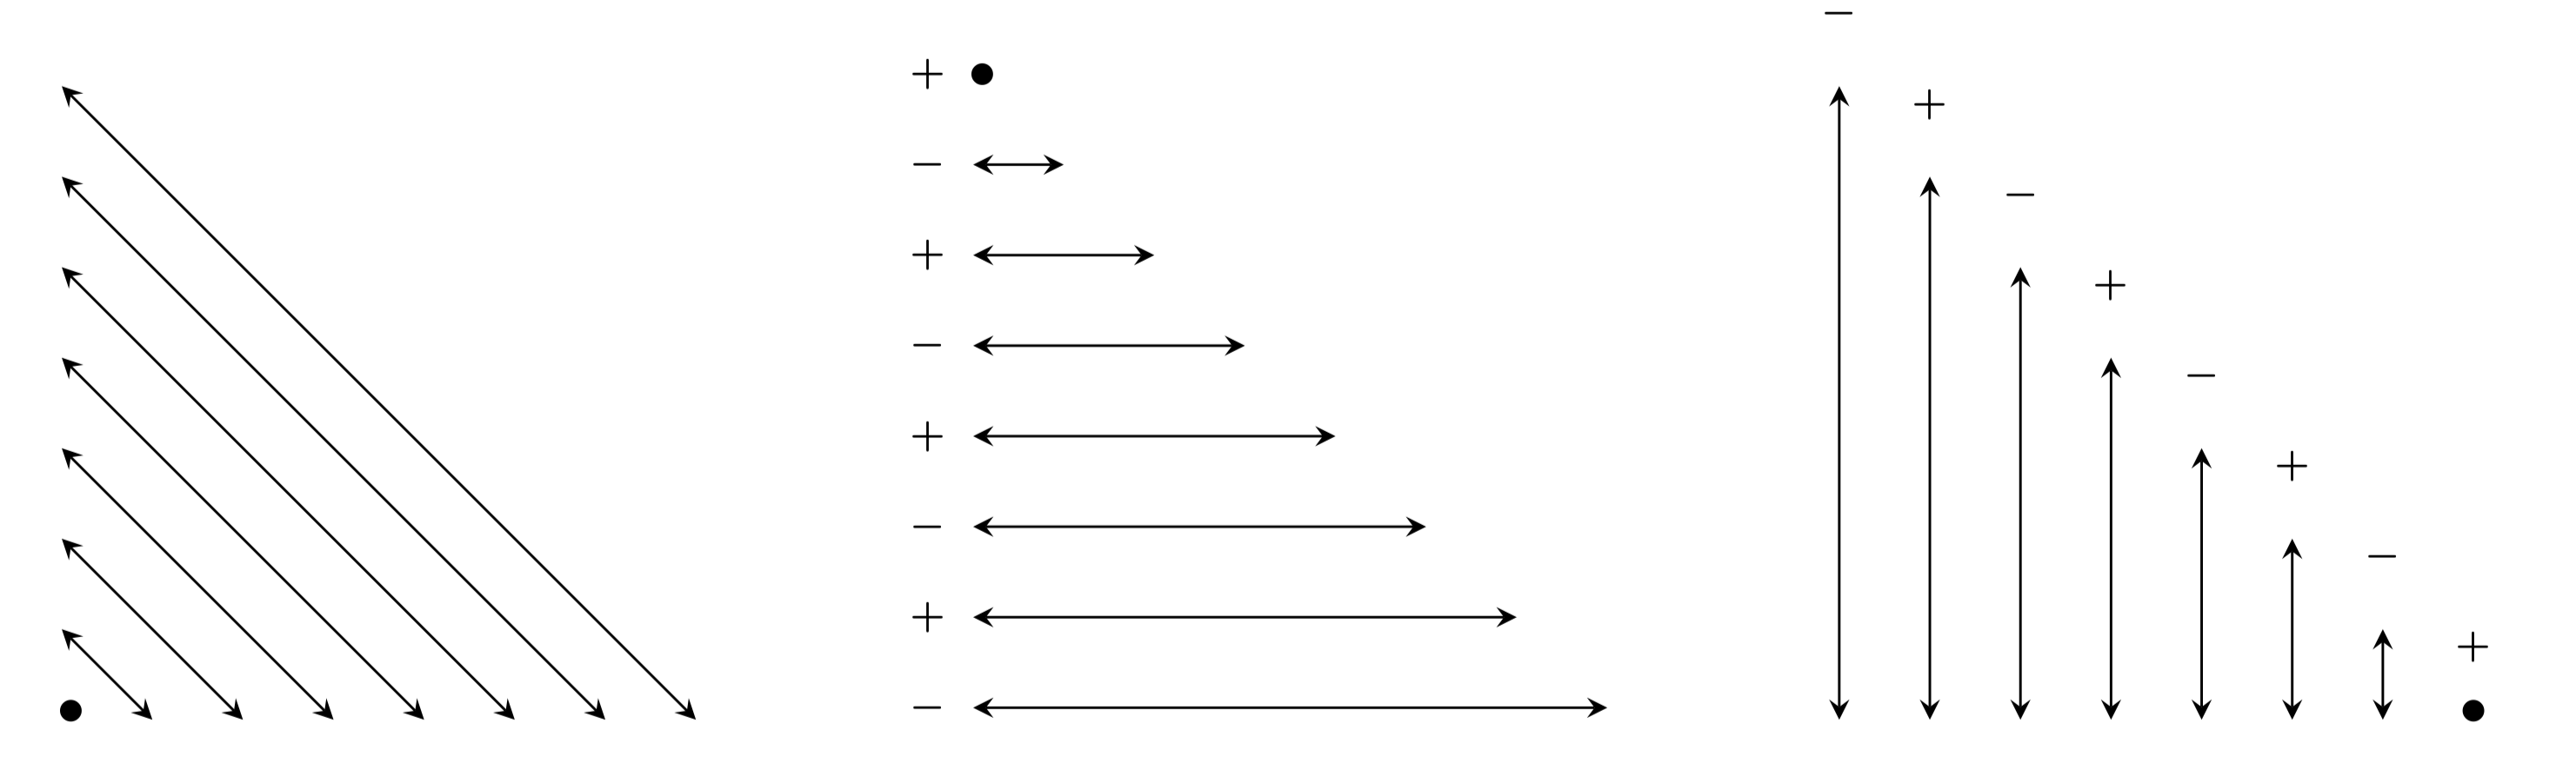
\includegraphics[width=\textwidth]{assets/group-action-s3.png}
    \caption{This illustration is taken from \cite{bik2022classifying}. The left most illustration shows mirroring the configuration with respect to the main diagonal. The middle illustration shows switching the order on the same row while also alternating the signs of the row. The right most illustration shows switching the order on the same column while also alternating the signs of the column.}
    \label{fig:group-action-s3}
\end{figure}

\section{Impossible Supports}\label{sec:impossible-supports}

Now, we show that specific supports cannot be the supports of valid integral outcomes. Hence, the title of this section \emph{Impossible Supports}. For instance, can we have an outcome whose support is only contained in \( S = \left\{ (0,0), (0,i) \right\} \) for some \( i \in \mathbb{N} \)? We will show that this is not possible.



\begin{proposition}\label{prop:impossible-support-23233243243423}
    Let \( d \in \mathbb{N} \), and \( i=0, \dots, d \). If \( S = \left\{ (0,i) \right\} \) and \( E = \left\{ 0 \right\} \), then \( A^{(d)}_{E,S} \) is invertible.
\end{proposition}

\begin{proof}
    We have \( A^{(d)}_{E,S} = \begin{bmatrix}
        1
    \end{bmatrix} \), which is invertible.
\end{proof}

\begin{proposition}\label{prop:impossible-support-232423}
    Let \( d \in \mathbb{N} \). Assume \( i,j=0, \dots, d \) with \( i < j \). If \( S = \left\{ (0,i), (0,j) \right\} \) and \( E = \left\{ 0,1 \right\} \), then \( A^{(d)}_{E,S} \) is invertible.
\end{proposition}

\begin{proof}
    We have \( A^{(d)}_{E,S} = \begin{bmatrix}
        1 & 1 \\ d-i & d-j
    \end{bmatrix} \), which is invertible.
\end{proof}

\begin{proposition}\label{prop:impossible-support-2}
    Let \( d \in \mathbb{N} \). Assume \( i,j,k=0, \dots, d \) with \( i < j < k \). If \( S = \left\{ (0,i), (0,j), (0,k) \right\} \) and \( E = \left\{ 0,1,2 \right\} \), then \( A^{(d)}_{E,S} \) is invertible.
\end{proposition}

\begin{proof}
    We have 
    \begin{align*}
        A^{(d)}_{E,S} = \begin{bmatrix}
            \binom{d-i}{0} & \binom{d-j}{0} & \binom{d-k}{0} \\
            \binom{d-i}{1} & \binom{d-j}{1} & \binom{d-k}{1} \\
            \binom{d-i}{2} & \binom{d-j}{2} & \binom{d-k}{2}
        \end{bmatrix} = \begin{bmatrix}
            1 & 1 & 1 \\
            d-i & d-j & d-k \\
            \frac{(d-i)(d-i-1)}{2} & \frac{(d-j)(d-j-1)}{2} & \frac{(d-k)(d-k-1)}{2}
        \end{bmatrix}.
    \end{align*}
    We substitute 
    \begin{align*}
        x &= d - i, \\
        y &= d - j, \\
        z &= d - k.
    \end{align*}
    Then, we see
    \begin{align*}
        \begin{bmatrix}
            1 & 0 & 0 \\
            0 & 1 & 0 \\
            0 & 1 & 2
        \end{bmatrix}A^{(d)}_{E,S} = \begin{bmatrix}
            1 & 1 & 1 \\
            x & y & z \\
            x^2 & y^2 & z^2
        \end{bmatrix}.
    \end{align*}
    The matrix on the right-hand side is invertible because it is a Vandermonde matrix. Thus, the pairing matrix \( A^{(d)}_{E,S} \) is invertible.
\end{proof}

\begin{proposition}\label{prop:impossible-support-2324223423123123}
    Let \( d \in \mathbb{N} \). Assume \( i,j=0, \dots, d \) with \( i < j \). Moreover, let \( k=0, \dots, d-1 \). If \( S = \left\{ (0,i), (0,j), (1,k) \right\} \), \( E = \left\{ 0,1,2 \right\} \), and \( i+j \neq 2k + 1 \), then \( A^{(d)}_{E,S} \) is invertible.
\end{proposition}

\begin{proof}
    We have 
    \begin{align*}
        A^{(d)}_{E,S} = \begin{bmatrix}
            \binom{d-i}{0} & \binom{d-j}{0} & \binom{d-k-1}{-1} \\
            \binom{d-i}{1} & \binom{d-j}{1} & \binom{d-k-1}{0} \\
            \binom{d-i}{2} & \binom{d-j}{2} & \binom{d-k-1}{1}
        \end{bmatrix} = \begin{bmatrix}
            1 & 1 & 0 \\
            d-i & d-j & d-k-1 \\
            \frac{(d-i)(d-i-1)}{2} & \frac{(d-j)(d-j-1)}{2} & \frac{(d-k-1)(d-k-2)}{2}
        \end{bmatrix}.
    \end{align*}
    We substitute 
    \begin{align*}
        x &= d - i, \\
        y &= d - j, \\
        z &= d - k - 1.
    \end{align*}
    Then, we see 
    \begin{align*}
        \begin{bmatrix}
            1 & 0 & 0 \\
            0 & 1 & 0 \\
            0 & 1 & 2
        \end{bmatrix}
        A^{(d)}_{E,S} \begin{bmatrix}
            1 & 1 & 0 \\
            0 & -1 & 0 \\
            0 & 0 & 1
        \end{bmatrix}
        \begin{bmatrix}
            1 & 0 & 0 \\
            0 & \frac{1}{x-y} & 0 \\
            0 & 0 & 1
        \end{bmatrix} = 
        \begin{bmatrix}
            1 & 0 & 0 \\
            x & 1 & 1 \\
            x^2 & x+y & 2z+1
        \end{bmatrix}.
    \end{align*}
    We see that the determinant is nonzero because \( x + y \neq 2z + 1 \) by \( i+j \neq 2k+1 \).
\end{proof}

\begin{remark}\label{rem:generality-jfknwejn}
    Without loss of generality, we may assume
\begin{align*}
    S &\subset \left\{ (i,j) \in V_d \mid i < \lvert S \rvert \right\}\\
    E &= \left\{ 0,1, \dots, \lvert S \rvert - 1 \right\}
\end{align*}
because the matrices \( A^{(d)}_{E,S} = A^{(d-\rho)}_{E - \rho, S - \rho} \) are equal, where \( \rho \coloneqq \min \left\{ E \cup \left\{ i \mid (i,j) \in S \right\} \right\} \) and \( E - \rho \coloneqq \left\{ (i - \rho, j) \mid (i,j) \in E \right\} \). This assumption allows us to apply the previous propostions to more general \( S \) and \( E \).
\end{remark}

\begin{example}
    Assume we have a configuration with support \( S = \left\{ (0,i), (0,j), (0,k) \right\} \) for \( 0 \leq i < j< k \leq d \). By Proposition \ref{prop:impossible-support-2}, we know that no valid integral nonzero outcome can have this support.

    Now, let us consider a configuration \( \mathbf{w} \) with support \( \mathrm{supp}(\mathbf{w}) \subset S \) such that \( S \) can be decomposed into \( S_1, \dots, S_l \) as described before. Let \( \ell = 1, \dots, l \). If \( S_\ell = \left\{ (x,i), (x,j), (x,k) \right\} \) for \( 0 \leq i < j< k \leq d \) and \( x \in \mathbb{N} \), then \( \mathbf{w} = \mathbf 0 \) by Proposition \ref{prop:impossible-support-2} and the previous comment on the generality of \( S \) and \( E \). 

    For instance, this configuration is not an outcome
    \begin{verbatim}
        *
        .  .
        .  .  *  
        .  .  .  .  
        .  .  .  *  .  
        .  .  .  .  .  .  
        .  .  .  *  .  .  .  
        *  .  .  *  .  .  .  .  
    \end{verbatim}
    where \( * \) denotes a non-zero entry. This is because for \( \lambda = (3,3,1,1) \) we have \( S_2 = \left\{ (3,0), (3,1), (3,3) \right\} \). Similarly, these configurations are not outcomes
    \begin{verbatim}
        *
        .  .
        .  .  *  
        .  .  .  .  
        .  .  .  .  .  
        .  .  .  *  .  .  
        .  .  .  *  .  .  .  
        *  .  .  *  .  .  .  .  
    \end{verbatim}
    \begin{verbatim}
        *
        .  .
        .  .  *  
        .  .  .  .  
        .  .  .  .  .  
        .  .  .  .  .  *  
        .  .  .  .  .  *  .  
        *  .  .  .  .  *  .  .  
    \end{verbatim}
    Of course, there are many more examples of impossible supports.
\end{example}